\section{复习}
\courseTime{Nov. 28, 2022. 10th, 1 of 4}

上周上机课的人最多。大家对这门课的感觉是什么?

今年是这门课的第三年,任课老师们一直在探索如何授课。目前来说,一直在推导基础知识,讲明白为止。

本课的内容是量化的原理和应用,理应更接近化学中的实际问题,但大部分内容是数学物理推导,远没有达到现阶段的量化。接下来两周的自旋、全同粒子,之后才是真正涉及到量化的基本算法。

先前的物化 1 已经给本课做了很好的铺垫。等各位到了研究生阶段,如果做理论或计算,还要学习量化。

% \textbf{量化的先修原理:}
我相信很多同学对量子力学一直是很懵懂,究其原因是微观粒子的和宏观物体的行为是完全不同的,如果利用直觉去理解量子力学是基本不可能的,只能借助数学工具。物理学家费曼言,``没有人能理解量子力学''。随着学习的深入,物理越来越像哲学,我们必须改变思维方式,以适应全新的物理图形,量化也是这样。

我们到目前为止,只是做了些准备工作。目的是,在日后的科研中碰到相关的知识,能够回想起来课上学过相关内容,就算不理解,也相信有途径去解决。前人已经总结了很多工具,去驯服复杂的微观粒子。

在力学实验中,沿着最速降线轨道的小球最先抵达终点,这是我们看得见、摸得着的实验。原子尺度的微观世界不可能看到,因为尺度远小于可见光波长,光学显微镜失效了。借助电子显微镜,分辨率可提升三个数量级,达到 $\SI{1E-10}{\metre} = \SI{0.1}{\nano\metre} = \SI{1}{\angstrom}$,从而``看到''原子世界。同样地,有方法研究宏观系统,也会有方法研究微观系统,总体来说是先易后难、螺旋上升的,这是唯物辩证法的规律之一。

硕士的量化课还有一学期,基本上是沿着本课的足迹,拓展到现阶段使用的量子化学方法。如果你不学本课,直接去听硕士的量化课,可能会感到深深的不安,因为所有的推导都是建立在本课的量子力学基础上的。当你熟练掌握量子力学、高等量子力学、数学物理方法等工具,一定会加深对量化的理解。

% 下一周涉及到量化。

% 2022-11-28 08:09:05  Wenbin Fan @FDU
上周是微扰。
从课程设置的角度来说,为什么要讲微扰?从课程设置的角度来说,并没有期望同学们可以理解,这与高中的``深挖坑''是不同的,高考要求我们熟练应用基础知识、技巧,本课的内容囫囵吞枣地理解即可。这并不是说忽略细节,而是要有更大的框架、更高的视角俯瞰本课的架构,当你遇到类似的问题之后要能反应过来用哪种方法求解。

% 希望囫囵吞枣地理解。
微扰的原理是什么?回到
第一节课,量子粒子的行为由量子力学基本原理保证,一次量子化中的基本原理是薛定谔方程。化学中的稳态是定态薛定谔方程,定态是不含时体系分离坐标和时间后的坐标部分。微观体系的性质全部由波函数决定。波函数是 $3N_{\text{atom}}$ 和时间的复函数,由薛定谔方程解出。

同学们相信牛顿力学,可能并不相信由理论演绎出的薛定谔方程。不管相信与否,微观的量子力学理论是经得起实验验证的,它是与宏观世界完全不同的。薛定谔为什么能提出 $\hat H \Psi = E \Psi$,因为他是当年的数学物理天才,是人们心中既定的诺奖获得者。当然,薛定谔方程不是凭空出来的,是联系了物理图像和波动方程得到的。当薛定谔的波动派遇上哥本哈根的矩阵派,双方并不能相互说服,直到狄拉克用数学推导证明了二者的等价性,才统一了量子力学的两大学派。(助教推荐上海市科技馆)

量子力学的创立,体现了人类超越造物主的强悍智慧。
% 后来爱因斯坦提出相对论 % 这个与课程不相关就不写了
当理论工具足够强大,是有可能超越现阶段的实验,去拓宽人类知识的边缘、打破科技前进的壁垒,这就是理论的强大之处。

哲学中的物质科学一直在强调实验和理论的\textbf{二元论},从实验中抽提出理论,理论再去解释实验。数学是超脱实验的,是由公理出发构造出的世界,体现着人类的最闪耀的智慧。

虽则人们对物质世界的认识,人们认识到了理论的局限性。特别是在复杂系统中,并不能总结出普适的规律。比如量子化学中,能精确求解真实系统的只有单电子原子。因此,\textbf{计算科学}应运而生,它很快成为了与实验、理论并驾齐驱的第三辆马车。

% % 2022-11-28 08:15:03  Wenbin Fan @FDU
% 科学的二元论是实验和理论。

% 数学是人类的最大智慧。

% 实验和理论

计算模拟,本质上是用\textbf{数值逼近},有必要对所研究的系统做近似。

我们讲过了\textbf{变分原理},它告诉我们,当不能精确求解时,如何逼近系统的能量,并给出了能量下界。当我们设定试探波函数,试探波函数构成了变分空间,变分法可给出在当前变分空间中的基态能量下限。如果变分空间包含真实的波函数,则变分法能求出真正的基态能量,如果不包括,则能求出最接近基态能量的下限能量。变分法的困难就在于,如何构造变分空间。

在求解单电子系统后,我们用变分法求解了两电子的波函数,此时变分参数取作有效核电荷 $Z$,进而确定原子核的屏蔽效应。不同的变分波函数,精度有高有低。

例题和作业都求解过了氦原子,我们用的波函数都是两个单电子波函数的乘积。考虑实际的情况,当电子 1 处在 $\vec r$ 处时,显然电子 2 无论如何都不可能处在 $\vec r$ 上,那么电子 2 在 $\vec r$ 处的密度(概率模方)应该为 0。尽管我们的尝试波函数包含了屏蔽效应,但是做不到上述这一点。一种更先进的变分函数,纳入了电子间的距离 $\frac1{r_{12}}$,由正的库伦排斥能可自然得到两电子距离为 0 时体系密度为 0。此方法的困难在于,引入 $\frac1{r_{12}}$ 后如何保证对称性,这在早年间有很多讨论。

我们看到,引入了恰当的变分参数后,可使得变分能量精确到小数点后七八位,这是很了不起的成就。可惜这种做法没有普适性,只能用在氦原子上。
% 比如求解氢原子的球谐函数也没有任何普适性。%% 这个话没错,放在这里逻辑不太连贯
因此,人们又发明了更加普适的变分方式——\textbf{线性变分},这个方法类似物化中讲过的原子轨道线性组合 linear combination of atomic orbitals (LCAO)。LCAO 背后对应的是,用原子轨道的线性组合当作基函数,利用变分法给出这些基函数系数的久期方程,进而解得基态能量。

% 2022-11-28 08:24:03  Wenbin Fan @FDU
从数学角度来说,原理就是这些,接下来讲一些数值模拟的原理。
上次上机课,助教讲了量化计算中最常用的 Gaussian-type function (GTF),并解释了它最常用是因为它容易求解。

GTF 有两个缺点,第一,靠近原子中心时原子轨道有尖点 cusp,GTF 很难描述,而 cusp 的行为是判断基组优劣的一个重要指标,人们用很多收缩(contracted,多个组合的)基函数描述 cusp。在 Gaussian 软件包中,关键词 \texttt{gfprint} 可输出基组信息,可以观察到,内层电子对应的 GFT 的 e 指数上的系数非常大,大到几千几万,这便是为了描述 cusp。

第二,氢原子 1s 轨道,e 指数上是一次方衰减,但 GTF 的 e 指数上是二次方衰减,这导致二者的渐进行为不一致,显然是指数上二次方衰减更快一些,导致 GTF 描述不好长程相互作用。
\suppInfo{基函数对比}{
    Slater 基函数接近真实,但不易算积分,现常用多个 Gaussian 函数拟合 Slater 基函数,形成 STO 基组。下面展示如何拟合,以及二者的差别。

归一化的 Slater-type function (STF) 为
\begin{align}
    \phi^{\text{SF}}_{\mathrm{1s}} (\zeta, \vec r) = \left(\frac{\zeta}\pi\right)^{1/2} \ee^{-\zeta | \vec r - \vec r_0 |},
\end{align}
归一化的 Gaussian-type function (GTF) 为
\begin{align}
    \phi^{\text{GF}}_{\mathrm{1s}} (\alpha, \vec r) = \left(\frac{2\alpha}\pi\right)^{3/4} \ee^{-\alpha | \vec r - \vec r_0 |^2}. 
\end{align}

取 $\zeta = 1$、$\vec r_0 = 0$ 的一维 STF,
\begin{align}
    \phi^{\text{SF}} = \pi^{-1/2} \ee^{-r},  
\end{align}
假设这是正确的。
再取 $L$ 个 GTF 去拟合 STF,得到的基组称为 STO-$L$G,具体表示为
\begin{align}
&\phi^{\text{CGF}} = \phi^{\text{GF}}(\alpha), \\
&\phi^{\text{CGF}} = A\phi^{\text{GF}}(\alpha) + B \phi^{\text{GF}}(\beta), \\
&\phi^{\text{CGF}} = A\phi^{\text{GF}}(\alpha) + B \phi^{\text{GF}}(\beta) + C \phi^{\text{GF}}(\gamma), 
\end{align}
接下来要优化 GTF 前面的系数,这称作优化基组。如何判断优化得足够好,或者说,所优化的目标函数是什么?因为 STF 和 GTF 都是归一化的,那么二者的重叠越大越好,也就是二者相乘的积分(重叠积分)越大越好,
\begin{align}
    S = \int \phi^{\text{SF}}_{1s} \phi^{\text{CGF}} \dd r .
\end{align}

经过数值算法优化,可得到
\begin{alignat}{3}
    &\text{STO-1G}\quad&\alpha = \num{0.270950} \quad&{}\\
    &\text{STO-2G}\quad&A = \num{0.678914} \quad &\alpha = \num{0.151623} \\
    & &B = \num{0.430129}\quad &\beta = \num{0.851819} \\
    &\text{STO-3G}\quad &A = \num{0.444635} \quad&\alpha = \num{0.109818} \\
    &&B = \num{0.535328}\quad&\beta = \num{0.405771}\\
    &&C = \num{0.154329}\quad&\gamma = \num{2.22766}
\end{alignat}
图像见图 \ref{fig:STO_GTO}。本部分内容来源于 Szabo ``Modern Quantum Chemistry'' \S 3.5.1。

如果想要拟合得更好,需要加入更多的 GTF。为了描述尖点,指数上的系数会非常大。
}
\begin{figure}[tbp]
    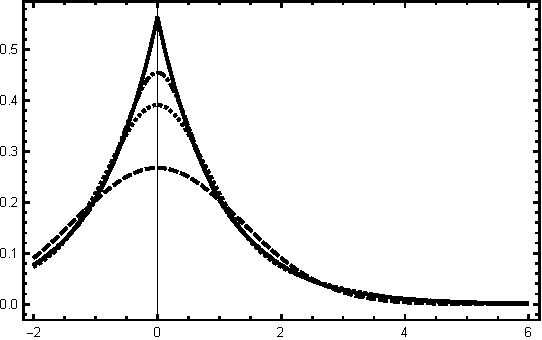
\includegraphics[height=3cm]{fig/STO_vs_GTO.pdf}
    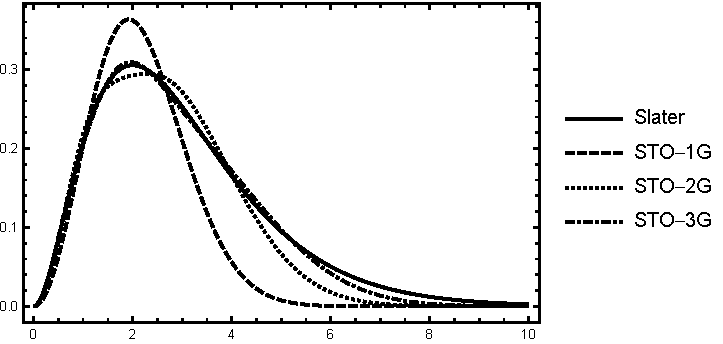
\includegraphics[height=3cm]{fig/STO_RDF.pdf}
    \caption{左图为基组,右图为基组的分布函数 $r^2\phi$}
    \label{fig:STO_GTO}
\end{figure}
% % MMA code
% Plot[{ST[1] r^2, 
%   GF[0.27095] r^2, (0.678914 GF[0.151623] + 
%      0.4330129 GF[0.851819]) r^2, (0.444635 GF[0.109818] + 
%      0.535328 GF[0.405771] + 0.154329 GF[2.22766]) r^2}, {r, 0, 10}, 
%  PlotTheme -> "Monochrome", Frame -> True, 
%  PlotLegends -> {"Slater", "STO-1G", "STO-2G", "STO-3G"}, 
%  PlotStyle -> Thick, FrameStyle -> Thickness[1/300], 
%  ImageSize -> Medium, PlotRange -> All]
% Export["STO_RDF.pdf", %]
%% 补充,Python 拟合 STO 基组:https://chc273.github.io/fitting-parameters-in-sto-lg/
%% 但是我用 MMA 就没有拟合出来,Szabo 书里的重叠积分没有 r^2 但应该有的。问题在于,两个 GTF 是完全等价的,总感觉这个搜索范围有点大(还有简并),很难把系数优化到最小 %% 放弃 %% 2022-11-29 19:48:03 Wenbin FAN @FDU

长程衰减速度不同,导致基组会影响渐进行为。
% 2022-11-28 08:29:15  Wenbin Fan @FDU
对电子比较弥散的系统,如阴离子束缚态,衰减快的 GTF 可能难以描述。阴离子的电子分布在原子的较外层,长程行为决定了体系跳出束缚态成为里德堡态的可能性。
% 非谐效应很重要 %% 跟非谐啥关系呢? %% 2022-11-29 21:19:20 Wenbin FAN @FDU
什么是阴离子束缚态?比如某体系有很强的偶极,当我们注入一个电子,电子最可能会出现在正极一侧。\ce{HF} 是一个典型,外侧可能会有一大团非常弥散的电子,这要求基组必须能正确描述波函数之间的长程相互作用,GTF 就会描述不好这种体系。
(助教注:这里应该是想说 dipole-bound state。加电场也可使得电子离域,当电场特别大时,电子可能会逸出,见 sobereva.com/570)

实际上,我们有办法直接用原子轨道基函数,那么为什么还要去拟合 GTF 呢?还是因为有解析结果。哪怕四中心积分存不下了,宁可 on-the-fly 即时计算,也要用 GTF。随着体系增大,四中心电子积分所需的内存量呈指数增长,一般来说是内存是放不下的,现在基本上都是即时计算的。

计算原子轨道基函数的积分有非常现实的困难。STO 不像 GTO 有解析解,STO 只能是格点积分。算一个 GTO 积分需要 \SI{1e-5}{\second},但数值的格点积分就需要 \SI{1e-2}{\second},慢了 \num{1000} 倍,这是根本不能承受的。现在确实有原子轨道基函数的程序,
% 比如 MS, Molcas (?) %% 搜了 atomic orbital integral direct 没有看到啥软件,这里就不写了 % 2022-11-29 22:21:27 Wenbin FAN @FDU
那么是用了什么技巧来节约时间呢?我们知道,四中心电子积分是四阶张量,如果用数学的方式把它降到三维或者二维,那积分结果直接就能放在内存里了。这种降维带来的优化是很恐怖的,比如原来的四中心积分需要 $\SI{100}{TB} = \SI{1e14}{bytes}$ 内存,降维成三维后只需要 $(\num{1e14})^{3/4}\,\text{bytes} = \SI{3.16e10}{bytes} = \SI{31.6}{GB}$,如果降维成二维,更是仅需 $\SI{1e7}{bytes} = \SI{10}{MB}$。原来只有超算才能算得动,现在台式机甚至是移动终端都可以算,这就是技术的进步,使得现阶段基组的选择空间就大了很多,这也是数值模拟中占比很高的研究内容。

返回来说,寻找基函数的时候另外还有个问题。量子力学基本假设说,
% 2022-11-28 08:33:55  Wenbin Fan @FDU
体系波函数最好是由具有相同边界条件的完备基展开,那么 Gaussian 型基函数是完备的吗?并不是的。完备集必须同时描述束缚态和解离态,但 GTF 显然不能描述解离态,我们刚讨论了电子完全解离的情况。
% 但 GTO 描述不了解离行为。
特别在高阶激发的时候,轨道形似解离态,波函数的行为像平面波,这是 GTO 无法描述的,GTO 不可能包含这样子的轨道。

对于一个原子的体系,可由角动量 $\hat L$ 展开得到完备集,是精确的。
% 【】完备的,角动量,指标展开得到完备基。
多个原子呢?需要用原子轨道的线性组合。两个原子上的原子轨道相互之间一定不会正交,因为有重叠,但是一个原子内的 GTF 可能是正交的。成键轨道就是两个原子上的原子轨道相互之间重叠很大,特别是共价键。
只要是分子体系,GTF 都不是完备基。
构造基组是个非常大的学问。

换句话说,如果我们遇到一个体系,现有的基函数表现不好,可否增加基函数来提高精度?实践经验告诉我们这是个非常有效的方法。再比如,post-Hartree--Fock 方法计算,波函数收敛非常非常慢,本质在于需要考虑 $1/r_{12}$ 的相互作用。
% 2022-11-28 08:40:07  Wenbin Fan @FDU
当两个电子靠近时,波函数有尖峰。现在所有的基组,都无法描述这个尖峰。轨道之间是相乘的,线性组合的原子轨道构造出的波函数,其中不会显式地出现 $1/r_{12}$,永远无法精确描述。如果增大基组,这导致数值不稳定、收敛困难。所以另有方法引入了距离,如二级微扰 MP2-F12、CCSD(T)-F12。

退回到基组本身,一直增加 GTF 到无穷多也可以是完备的,但不能实现。有没有完备基组呢?有的,凝聚态物理中常用的第一性软件 VASP 中用到的\textbf{平面波}基组就是完备的,而且平面波的动量是连续的。注意到 VASP 要求输入截断能 cutoff,这相当于我们取了从 0 到截断能这一段的平面波去展开波函数,如果不足以描述,增大截断能即可。

对于分子而言,理论上可通过平面波的组合以给出定域 local 的形式,
因为平面波是全空间等价的。
% 平面波可以描述尖点,但需要无穷多个平面波。
平面波的优点是适合描述长程行为,但是同样地靠近原子核的 cusp 难以描述。
% 【】
平面波如何处理内核电子?这就需要\textbf{赝势} pseudo-potential 将内层电子简化,本来内层电子的势能有剧烈变化,赝势则是用平滑的函数构造了内层电子并连接到价电子部分。

此外,对于同一个体系,所需的平面波数量要远大于 Gaussian 型基函数,比如一氧化碳 CO,只需要 20 个 GTF,但需要 \num{20000} 个平面波。
如此大量的基函数,会产生一个超大的稠密矩阵,对角化稠密矩阵也是个困难的问题。不同领域用不同的基函数,都有各自的难点。很自然地,有课题组开发了平面波和 GTF 结合的基组,使得 GTF 能嵌入到平面波基组中,这也是长久以来的研究方向。
% 有没有既又?小波基组,【?】混合基组。这有很多方向。
我们课题组也有过该领域的研究,如果感兴趣,欢迎加入我们。


从科学研究范式来说,1500 年前的炼金术是实验科学,牛顿等人构建起的经典物理是理论科学。从物理到化学到工程应用,实践越来越需要理论的指导。
% 是模拟科学。

从 1950 年开始,计算机开始发展。如果没有现代计算机、没有计算科学,人们不可能对微观世界有定量的认识,三个原子已经极难手工计算了,老一辈科学家手算氢弹是很令人敬佩的。计算化学已经成为了独立的学科,是一种重要的研究方式。

最新的研究方式是大数据科学、人工智能,这是一个不断进化的过程,背后反映出数学理论的进步、计算硬件的发展。
% 2022-11-28 08:49:59  Wenbin Fan @FDU
% 掌控大自然。数学工具,计算工具,基于各种工具的研究范式。
有了各种理论和工具,才能更好地理解和掌控大自然。
% 当然技术是双刃剑



\courseTime{Nov 28, 10th, 2 of 4}
继续上课。

微扰相对于变分,是另外一套用来数值逼近的方式。
微扰和变分都是计算科学中重要的原理,下周还会讲密度泛函理论,再下节课讲多电子体系。多电子体系又是另外一个世界,还要引入自旋,从多电子体系开始才算是真正买入量化计算的门槛。很可惜,我们这门课只能讲到密度泛函理论,后续内容在研究生的量化课上会继续讲。

薛定谔方程不能精确求解,变分法的目标是寻找尝试波函数。近期数学领域张益唐教授的工作非常热门,其核心思想是,将原来的大海捞针,变成了在大海的子集中找到一根针,后人可不断扩大这个子集。变分有点像大海捞针,不断构造合适的尝试波函数,实际上两个电子的变分已经很困难了,何况多电子体系。

% 变分法,不断扩大【】

微扰法告诉我们,复杂的体系没法求解,但是可以找到一个跳板去间接处理。假设有个体系
\begin{align}
    \hat H_0 \psi_n^{(0)} = E_n^{(0)} \psi_n^{(0)}
\end{align}
可以精确求解,同时 $\hat H - \hat H_0 = \hat H'$ 是微小差别,那么可微扰求解。构造微扰途径,线性的是最常用的,相当于 $\hat H_0$ 和真实体系的纽带,
\begin{align}
    \hat H(\lambda) = \hat H_0 + \lambda H',
\end{align}
因此薛定谔方程可以写为
\begin{align}
    \hat H(\lambda) \psi_n(\lambda) = E_n(\lambda) \psi_n(\lambda), 
\end{align}
波函数和能量可以展开为
\begin{align}
    &\psi_n(\lambda) = \psi_n^{(0)} + \lambda \psi_n^{(1)} + \lambda^2 \psi_n^{(2)} + \cdots, \\
    &E_n(\lambda) = E_n^{(0)} + \lambda E_n^{(1)} + \lambda^2 E_n^{(2)} + \cdots, 
\end{align}
其中,上标 $(k)$ 表示 $k$ 级校正。

\textbf{非简并的微扰理论},
\begin{align}
    &E_n^{(1)} = \langle \psi_n^{(0)} | \hat H' | \psi_n^{(0)} \rangle = H_{nn}', \quad H_{ij} = \langle \psi_i^{(0)} | \hat H' | \psi_j^{(0)} \rangle, \\
    &\psi_n^{(1)} = \sum_{j\neq n} \frac{\langle \psi_j^{(0)} | \hat H | \psi_n^{(0)} \rangle} {E_n^{(0)} - E_j^{(0)}} \psi_j^{(0)} = \sum_{j\neq n} \frac{H'_{jn}}{E_n^{(0)} - E_j^{(0)}} \psi_j^{(0)},\\
    &E_n^{(2)} = \langle \psi_n^{(0)} | \hat H | \psi_n^{(1)} \rangle = 
    \sum_{j\neq n} \frac{|H_{jn}'|^2}{E_n^{(0)} - E_j^{(0)}}, 
\end{align}

% 同学问,为什么各级微扰波函数之间正交?因为一级微扰波函数是用零级未微扰波函数展开的,所以相互之间没有关系。
% 拉格朗日展开
\section{氦原子的激发态}
氦原子的电子基态的微扰,
\begin{align}
    \hat H_0 = - \frac{\hbar^2}{2m_{\mathrm e}} (\hat \nabla_1^2 + \hat \nabla_2^2) - \frac{2e^2}{r_1} - \frac{2e^2}{r_2}, \quad \hat H' = \frac{e^2}{r_{12}},
\end{align}
波函数和能量
\begin{align}
    &\psi_1^{(0)}(\vec r_1, \vec r_2) = \psi_{\text{1s}} (\vec r_1) \psi_{\text{1s}} (\vec r_2) = \frac 1\pi \left(\frac2{a_0}\right)^3 \ee^{-\frac2{a_0}(\vec r_1 + \vec r_2)} = \psi_{\text{1s}}^2,
    \\
    &E_1^{(1)} =  \langle \psi_1^{(0)} | \hat H' | \psi_1^{(0)} \rangle = \frac 54 \frac{\hbar^2}{m_\mathrm{e} a_0^2}, 
\end{align}
则
\begin{align}
    &E_1 \approx  E_1^{(0)} + E_1^{(1)} = \left(-4 + \frac54\right) \frac{\hbar^2}{m_\mathrm{e}a_0^2} = -2.75 \,{\hbar^2}{m_\mathrm{e}a_0^2},\\
    &\psi_1 \approx  \psi_1^{(0)} + \psi_1^{(1)} = \psi_1^{(0)} + \sum_{j\neq1} \frac{H'_{j1}}{E_1^{(0)} - E_j^{(0)}} \psi_j^{(0)},
\end{align}

% 2022-11-28 09:19:18  Wenbin Fan @FDU
% 【图】
% n=2 不止这两个轨道是简并的。
\begin{table}[tp]
\centering
\caption{氦原子的电子排布}
\label{tab:he_electron_pop}
\begin{tabular}{>{\centering\arraybackslash }m{5mm} >{\centering }m{5mm} >{\centering }m{12mm} >{\centering }m{42mm} >{\centering\arraybackslash }m{2cm}}
\hline
No. & $n$ & 排布 & 图示 & 布居 \\
\hline
1 & 1 & 1s$^2$ & 
\begin{tikzpicture}[scale=0.7]
    \newcommand\w{0.8}
    \renewcommand\s{0.3}
    \newcommand\labelshift{0.4}
    \newcommand\arrowlenhalf{0.5}
    
    \fill[white, opacity=0.0] (0, 0-\arrowlenhalf-0.5) rectangle (5*\w+4*\s, 1+\arrowlenhalf);

    \draw (0,0) -- (\w,0);
    \node[below] at (\w/2,0-\labelshift) {1s}; 
    
    \newcommand\ess{0.6}
    \draw (\w+\s,\ess) -- (2*\w+\s,\ess);
    \node[below] at (\w+\s+\w/2, \ess-\labelshift) {2s};
    
    \newcommand\ep{1}
    \draw (2*\w+2*\s, \ep) -- (3*\w + 2*\s, \ep);
    \node[below] at (2*\w+2*\s+\w/2, \ep-\labelshift) {2p$_x$};
    \draw (3*\w+3*\s, \ep) -- (4*\w + 3*\s, \ep);
    \node[below] at (3*\w+3*\s+\w/2, \ep-\labelshift) {2p$_y$};
    \draw (4*\w+4*\s, \ep) -- (5*\w + 4*\s, \ep);
    \node[below] at (4*\w+4*\s+\w/2, \ep-\labelshift) {2p$_z$};
    
    % draw arrow
    \draw[->, thick, -Latex] (\w/2+0.1, \arrowlenhalf) -- (\w/2+0.1, -\arrowlenhalf);
    \draw[->, thick, -Latex] (\w/2-0.1, -\arrowlenhalf) -- (\w/2-0.1, \arrowlenhalf);
\end{tikzpicture}
&
1s(1)\,1s(2) 
\\
2 & 2 & 1s\,2s  & 
\begin{tikzpicture}[scale=0.7]
    \newcommand\w{0.8}
    \renewcommand\s{0.3}
    \newcommand\labelshift{0.4}
    \newcommand\arrowlenhalf{0.5}
    
    % \fill[white, opacity=0.0] (0, 0-\arrowlenhalf-0.5) rectangle (5*\w+4*\s, 1+\arrowlenhalf);

    \draw (0,0) -- (\w,0);
    \node[below] at (\w/2,0-\labelshift) {1s}; 
    
    \newcommand\ess{0.6}
    \draw (\w+\s,\ess) -- (2*\w+\s,\ess);
    \node[below] at (\w+\s+\w/2, \ess-\labelshift) {2s};
    
    \newcommand\ep{1}
    \draw (2*\w+2*\s, \ep) -- (3*\w + 2*\s, \ep);
    \node[below] at (2*\w+2*\s+\w/2, \ep-\labelshift) {2p$_x$};
    \draw (3*\w+3*\s, \ep) -- (4*\w + 3*\s, \ep);
    \node[below] at (3*\w+3*\s+\w/2, \ep-\labelshift) {2p$_y$};
    \draw (4*\w+4*\s, \ep) -- (5*\w + 4*\s, \ep);
    \node[below] at (4*\w+4*\s+\w/2, \ep-\labelshift) {2p$_z$};
    
    % draw arrow
    \draw[->, thick, -Latex] (\w/2, -\arrowlenhalf) -- (\w/2, \arrowlenhalf);
    \draw[->, thick, -Latex] (\w+\s+\w/2, \ess+\arrowlenhalf) -- (\w+\s+\w/2, \ess-\arrowlenhalf);
\end{tikzpicture}
& 1s(1)\,2s(2) \\
3 & 2 & 1s\,2s  & 
\begin{tikzpicture}[scale=0.7]
    \newcommand\w{0.8}
    \renewcommand\s{0.3}
    \newcommand\labelshift{0.4}
    \newcommand\arrowlenhalf{0.5}
    
    % \fill[white, opacity=0.0] (0, 0-\arrowlenhalf-0.5) rectangle (5*\w+4*\s, 1+\arrowlenhalf);

    \draw (0,0) -- (\w,0);
    \node[below] at (\w/2,0-\labelshift) {1s}; 
    
    \newcommand\ess{0.6}
    \draw (\w+\s,\ess) -- (2*\w+\s,\ess);
    \node[below] at (\w+\s+\w/2, \ess-\labelshift) {2s};
    
    \newcommand\ep{1}
    \draw (2*\w+2*\s, \ep) -- (3*\w + 2*\s, \ep);
    \node[below] at (2*\w+2*\s+\w/2, \ep-\labelshift) {2p$_x$};
    \draw (3*\w+3*\s, \ep) -- (4*\w + 3*\s, \ep);
    \node[below] at (3*\w+3*\s+\w/2, \ep-\labelshift) {2p$_y$};
    \draw (4*\w+4*\s, \ep) -- (5*\w + 4*\s, \ep);
    \node[below] at (4*\w+4*\s+\w/2, \ep-\labelshift) {2p$_z$};
    
    % draw arrow
    \draw[->, thick, -Latex] (\w/2, \arrowlenhalf) -- (\w/2, -\arrowlenhalf);
    \draw[->, thick, -Latex] (\w+\s+\w/2, \ess-\arrowlenhalf) -- (\w+\s+\w/2, \ess+\arrowlenhalf);
\end{tikzpicture}
& 2s(1)\,1s(2) \\
4 & 2 & 1s\,2p  & 
\multirow{3}{*}{
\begin{tikzpicture}[scale=0.7]
    \newcommand\w{0.8}
    \renewcommand\s{0.3}
    \newcommand\labelshift{0.4}
    \newcommand\arrowlenhalf{0.5}
    
    \fill[white, opacity=0.0] (0, 0-\arrowlenhalf-2) rectangle (5*\w+4*\s, 1+\arrowlenhalf);

    \draw (0,0) -- (\w,0);
    \node[below] at (\w/2,0-\labelshift) {1s}; 
    
    \newcommand\ess{0.6}
    \draw (\w+\s,\ess) -- (2*\w+\s,\ess);
    \node[below] at (\w+\s+\w/2, \ess-\labelshift) {2s};
    
    \newcommand\ep{1}
    \draw (2*\w+2*\s, \ep) -- (3*\w + 2*\s, \ep);
    \node[below] at (2*\w+2*\s+\w/2, \ep-\labelshift) {2p$_x$};
    \draw (3*\w+3*\s, \ep) -- (4*\w + 3*\s, \ep);
    \node[below] at (3*\w+3*\s+\w/2, \ep-\labelshift) {2p$_y$};
    \draw (4*\w+4*\s, \ep) -- (5*\w + 4*\s, \ep);
    \node[below] at (4*\w+4*\s+\w/2, \ep-\labelshift) {2p$_z$};
    
    % draw arrow
    \draw[->, thick, -Latex] (\w/2, -\arrowlenhalf) -- (\w/2, \arrowlenhalf);
    \draw[->, thick, -Latex] (2*\w+2*\s+\w/2, \ep+\arrowlenhalf) -- (2*\w+2*\s+\w/2, \ep-\arrowlenhalf);
    \draw[->, thick, -Latex, red] (3*\w+3*\s+\w/2, \ep+\arrowlenhalf) -- (3*\w+3*\s+\w/2, \ep-\arrowlenhalf);
    \draw[->, thick, -Latex, blue] (4*\w+4*\s+\w/2, \ep+\arrowlenhalf) -- (4*\w+4*\s+\w/2, \ep-\arrowlenhalf);
\end{tikzpicture}
}
& 1s(1)\,2p$_x$(2) \\
5 & 2 & 1s\,2p& & 1s(1)\,{\color{red}2p$_y$(2)}\\
6 & 2 & 1s\,2p& & 1s(1)\,{\color{blue}2p$_z$(2)}\\
\rule{0pt}{2mm}\\
7 & 2 & 1s\,2p  & 
\multirow{3}{*}{
\begin{tikzpicture}[scale=0.7]
    \newcommand\w{0.8}
    \renewcommand\s{0.3}
    \newcommand\labelshift{0.4}
    \newcommand\arrowlenhalf{0.5}
    
    \fill[white, opacity=0.0] (0, 0-\arrowlenhalf-0.5) rectangle (5*\w+4*\s, 1+\arrowlenhalf);

    \draw (0,0) -- (\w,0);
    \node[below] at (\w/2,0-\labelshift) {1s}; 
    
    \newcommand\ess{0.6}
    \draw (\w+\s,\ess) -- (2*\w+\s,\ess);
    \node[below] at (\w+\s+\w/2, \ess-\labelshift) {2s};
    
    \newcommand\ep{1}
    \draw (2*\w+2*\s, \ep) -- (3*\w + 2*\s, \ep);
    \node[below] at (2*\w+2*\s+\w/2, \ep-\labelshift) {2p$_x$};
    \draw (3*\w+3*\s, \ep) -- (4*\w + 3*\s, \ep);
    \node[below] at (3*\w+3*\s+\w/2, \ep-\labelshift) {2p$_y$};
    \draw (4*\w+4*\s, \ep) -- (5*\w + 4*\s, \ep);
    \node[below] at (4*\w+4*\s+\w/2, \ep-\labelshift) {2p$_z$};
    
    % draw arrow
    \draw[->, thick, -Latex] (\w/2, \arrowlenhalf) -- (\w/2, -\arrowlenhalf);
    \draw[->, thick, -Latex] (2*\w+2*\s+\w/2, \ep-\arrowlenhalf) -- (2*\w+2*\s+\w/2, \ep+\arrowlenhalf);
    \draw[->, thick, -Latex, red] (3*\w+3*\s+\w/2, \ep-\arrowlenhalf) -- (3*\w+3*\s+\w/2, \ep+\arrowlenhalf);
    \draw[->, thick, -Latex, blue] (4*\w+4*\s+\w/2, \ep-\arrowlenhalf) -- (4*\w+4*\s+\w/2, \ep+\arrowlenhalf);
\end{tikzpicture}
}
& 2p$_x$(1)\,1s(2) \\
8 & 2 & 1s\,2p& & {\color{red}2p$_y$(1)}\,1s(2)\\
9 & 2 & 1s\,2p& & {\color{blue}2p$_z$(1)}\,1s(2)\\
\rule{0pt}{0pt}  \\ % add vertical space
\hline
\end{tabular}
\end{table}

表格 \ref{tab:he_electron_pop} 中列出了氦原子的基态和部分激发态。我们已经求解了基态波函数和能量,那么怎么求解激发态呢?
% 现在我们要问个问题。1s-2s、1s-2p 的屏蔽效应不一样,那么还能简并吗?如何求解氦原子的第一激发态?
从物理上来说,1s 轨道对于 2s、对于 2p 轨道的屏蔽效应是不同的,考虑了这种屏蔽效应之后,原来简并的能级就不简并了。下面尝试求解第一激发态,这与后面的自旋有一点关联。

上次课讲过了简并能级的微扰法,需要重新讲,还是直接给答案?(同学:直接给吧,时间不太够)

从表格 \ref{tab:he_electron_pop} 已经得到了激发态的八重简并,对应序号 2---9。那么一级微扰波函数,需要用这 8 个简并态来展开。下面写出这 8 个零级激发的贡献,
\begin{alignat}{2}
&\psi_1^{(0)} = \mathrm{1s(1)\,2s(2)} &\quad \text{偶偶} \\
&\psi_2^{(0)} = \mathrm{2s(1)\,1s(2)} &\quad \text{偶偶}
\end{alignat}
\begin{alignat}{2}
&\psi_3^{(0)} = \mathrm{1s(1)\,2p}_x(2) &\quad \text{偶奇} \\
&\psi_4^{(0)} = \mathrm{2p}_x(1)\,2\mathrm{s}(2) &\quad \text{奇偶}
\end{alignat}
\begin{alignat}{2}
&\psi_5^{(0)} = \mathrm{1s(1)\,2p}_y(2) &\quad \text{偶奇} \\
&\psi_6^{(0)} = \mathrm{2p}_y(1)\,2\mathrm{s}(2) &\quad \text{奇偶}
\end{alignat}
\begin{alignat}{2}
&\psi_7^{(0)} = \mathrm{1s(1)\,2p}_z(2) &\quad \text{偶奇} \\
&\psi_8^{(0)} = \mathrm{2p}_z(1)\,2\mathrm{s}(2) &\quad \text{奇偶}
\end{alignat}
% \begin{align}
%     \psi_1^{(0)} = 1s(1) \ 2s(2), \quad & \psi_5^{(0)} = 1s(2) \ 2p_y(2), \\
%     [][]
% \end{align}
其中第八个波函数的表达式为
\begin{align}
    \psi_8^{(0)} = \frac1{(4\pi)^{1/2}} \left(\frac Z{a_0}\right)^{5/2} r_1 \ee^{-\frac{Z r_1}{2a_0}} \cos\theta_1 \frac1{\sqrt{\pi}} \left(\frac{Z}{a_0}\right)^{3/2} \ee^{-\frac{Zr_2}{a_0}}, 
\end{align}

这些内容看起来很复杂,实际上并不惜要同学们记住,如果考到了会给出公式的作为任课教师更希望同学们学到的是思维方式。日后看文献也是同理,文献不可能全部看完的,更不可能都记住,必须要在文献中找到找到所需的知识点,并尽量用起来。
% 【看文献也是】

简并的波函数描述成
\begin{align}
    \psi_n^{(1)} = \sum_{i=1}^8 c_in \psi_i^{(0)}, \quad i=1,\cdots,8,
\end{align}
其中的展开系数 $c_{in}$ 对应久期方程,
\begin{align}
    \left|\begin{matrix}
        H'_{11} - E_1^{(1)} & H_{12}' & \cdots & H'_{18} \\
        H'_{21} & H'_{22} - E_2^{(1)} & \cdots & H'_{28} \\
        \vdots & \vdots & \ddots & \vdots \\
        H'_{81} & H'_{82} & \cdots & H'_{88} - E_8^{(1)}
    \end{matrix}\right| = 0
\end{align}
我们需要求解其中的 $H_{ij}'$。
% 公式在前面已经给出来了。

这个 $8\times8$ 的矩阵太复杂,先做一些化简。(1) 容易证明 8 个轨道是正交归一的,有
\begin{align}
    \langle \psi_i^{(0)} | \psi_j^{(0)} \rangle = \delta_{ij}, \quad i,j = 1, 2, \cdots, 8. 
\end{align}
(2) 实空间的厄米算符,有
\begin{align}
    H_{ij} = (H_{ji}')^* = H_{ji}'. 
\end{align}
(3) 利用宇称(对称性),以
\begin{align}
    H'_{13} = \left\langle \mathrm{1s(1) \, 2s(2)} \middle | \frac{e^2}{r_{12}} \middle| \mathrm{1s(1)\,2p}_x(2) \right\rangle
\end{align}
为例,
对其中一个坐标分量 $x$ 反演,即 $x\rightarrow -x$,有
\begin{align}
\psi_{\mathrm{1s}}^* (+x_1, y_1, z_1) &\rightarrow \psi_{\mathrm{1s}}^* (-x_1, y_1, z_1) \\
\psi_{\mathrm{2s}}^* (+x_2, y_2, z_2) &\rightarrow \psi_{\mathrm{2s}}^* (-x_2, y_2, z_2) \\
\frac{e^2}{r_{12}} &\rightarrow \frac{e^2}{r_{12}} \\
% {\sqrt{(x_1-x_2)^2 + (y_1-y_2)^2 + (z_1-z_2)^2}}
\psi_{\mathrm{1s}} (+x_1, y_1, z_1) &\rightarrow \psi_{\mathrm{1s}} (-x_1, y_1, z_1) \\
\psi_{\mathrm{2p}_x} (+x_2, y_2, z_2) &\rightarrow \psi_{\mathrm{2p}_x}(-x_2, y_2, z_2) \\ 
\end{align}
注意到其中 $\psi_{2\mathrm{p}_x}$ 是关于 $yOz$ 平面对称的,反演后波函数为负。因为奇函数在对称区间上的积分为 0,所以这个积分为 0。

由此,将大矩阵分解成了 4 个小矩阵,
\begin{align}
\left|
\begin{matrix}
\begin{matrix}
b_{11} & H_{12}' \\ H_{21}' & b_{22}
\end{matrix} & {} & {} & 0 \\
{} & \begin{matrix}
    b_{33} & H_{34}' \\ H_{43}' & b_44
\end{matrix} & {} & {} \\
{} & {} &
\begin{matrix}
    b_{55} & H_{56}' \\ H_{65}' & b_{66}
\end{matrix} & {} \\
0& {} & {} &\begin{matrix}
    b_{77} & H_{78}' \\ H_{87}' & b_{88}
\end{matrix}
\end{matrix}
\right|=0,
\end{align}
其中
\begin{align}
    b_{nn} = H'_{nn} - E_n^{(1)}, \quad n=1,\cdots,8,
\end{align}
整个大的行列式为 0,只需要其中四个小的行列式为 0。比如第一个 $2\times2$ 的行列式,
\begin{align}
    \label{eq:he_excited_2times2}
    \left|\begin{matrix}
        H_{11}'-E_1^{(1)} & H_{12}' \\
        H_{21}' & H_{22}' - E_2^{(1)}
    \end{matrix}
    \right|=0. 
\end{align}

余下的内容下午再讲。徐老师今年特别忙,所以大部分课由张颖老师完成。在张老师的强烈建议下,徐昕老师会来讲最后一次课,内容是 DFT。未来几次课,张老师会快速讲一遍自旋、密度泛函理论的基本概念。上机操作的 QC 队列会保留到本学期结束。

\courseTime{3 of 4, 10th}
% 3 of 4
% 上午接着讲了微扰:简并微扰的应用。
我们现在的目的是求 He 原子的第一激发态。采用无相互作用的波函数作为未微扰波函数。

下面显式写出 $H_{11}'$ 和 $H_{22}'$ 的表达式,
\begin{align}
&H_{11}' = \left\langle \mathrm{1s(1)\,2s(2)} \middle| \frac{e^2}{r_{12}} \middle| \mathrm{1s(1)\,2s(2)} \right\rangle, \\
&H_{22}' = \left\langle \mathrm{2s(1)\,1s(2)} \middle| \frac{e^2}{r_{12}} \middle| \mathrm{2s(1)\,1s(2)} \right\rangle, 
\end{align}
% 2022-11-28 13:35:02  Wenbin Fan @FDU
很明显,
\begin{align}
    H_{11}' = H_{22}', \quad H_{33}' = H_{44}', \quad H_{55}' = H_{66}', \quad H_{77}' = H_{88}',
\end{align}
这里比较好理解,以 $H'_{11} = H'_{22}$ 来说,它是指「电子1 在 1s、电子2 在 2s」和「电子 2 在 1s、电子 1 在 1s」这两种组态是等价的。

以 $H_{11}'$ 为例,展开为
\begin{align}
    H_{11}' &= \iint |\psi_{\text{1s}}(\vec r_1)|^2 |\psi_{\text{2s}}(\vec r_2)|^2 \frac{e^2}{r_{12}} \,\dd\vec r_1 \dd\vec r_2 \\
    & = \iint \rho(\vec r_1) \rho(\vec r_2) \,\dd\vec r_1 \dd\vec r_2,
\end{align}
其中的 $\rho$ 是密度分布,
\begin{align}
    \rho(\vec r_1) = |\psi_{\text{1s}}(\vec r_1)|^2,
    \quad 
    \rho(\vec r_2) = |\psi_{\text{2s}}(\vec r_2)|^2,
\end{align}
由此密度视角,$H_{11}'$ 可理解为两电子间的库伦相互作用,用 $J$ 表示,即
\begin{align}
    H'_{11} = J_{\text{1s\,2s}}, \quad H_{22}' = J_{\text{2s\,1s}},
\end{align}
称作\boldtext{库伦积分}。对于 $H_{12}'$,其表达式为
\begin{align}
H_{12}' &= \iint \psi_{\text{1s}}^*(\vec r_1) \psi_{\text{2s}} (\vec r_1) \frac{e^2}{r_{12}} \psi_{\text{2s}}^*(\vec r_2) \psi_{\text{1s}} (\vec r_1) \,\dd\vec r_1 \dd\vec r_2 \equiv K_{\text{1s\,2s}},
\end{align}
定义其为\boldtext{交换积分}。总结为,
\begin{align}
&\text{库伦积分}\quad 
J_{mn} \equiv \left\langle f_m(1) f_n(2) \middle| \frac{e^2}{r_{12}} \middle| f_m(1)f_n(2) \right\rangle, \\
&\text{交换积分}\quad K_{mn} \equiv \left\langle f_m(1) f_n(2) \middle| \frac{e^2}{r_{12}} \middle| f_n(1)f_m(2) \right\rangle. 
\end{align}

继续求解上面 $2\times2$ 的小矩阵 \eqref{eq:he_excited_2times2},根据两种积分的定义,有
% % 2022-11-28 13:45:42  Wenbin Fan @FDU
% 对角元都相等。全空间积分,先后顺序无关。
\begin{align}
    \left|\begin{matrix}
        J_{\text{1s\,2s}} - E^{(1)} & K_{\text{1s\,2s}} \\
        K_{\text{1s\,2s}} & J_{\text{1s\,2s}} - E^{(1)}
    \end{matrix}\right| = 0
\end{align}
按照两种积分的定义,显然有
\begin{align}
    K_{mn} = K_{nm}, \quad J_{mn} = J_{nm},
\end{align}
那么容易解得这个行列式
\begin{align}
E_1^{(1)} = J_{\text{1s\,2s}} - K_{\text{1s\,2s}}, \quad E_2^{(2)} = J_{\text{1s\,2s}} + K_{\text{1s\,2s}},
\end{align}
% 2022-11-28 13:49:31  Wenbin Fan @FDU
因此,现在已经分解开了
% 【见照片】
表格 \ref{tab:he_electron_pop} 中第二个、第三个激发态
的两种简并。

% 2022-11-28 13:53:40  Wenbin Fan @FDU
求解出了能量,那么激发态的展开系数 $c$ 也可求得两种情况,进而得到一级微扰波函数为
% 【这个 c 是前面定义处的展开系数】
\begin{align}
&\psi_1^{(1)} = \frac1{\sqrt2} \big[ \mathrm{1s(1)\,2s(2) - 2s(1)\,1s(2)} \big], \\
&\psi_2^{(1)} = \frac1{\sqrt2} \big[ \mathrm{1s(1)\,2s(2) + 2s(1)\,1s(2)} \big]. 
\end{align}
\suppInfo{矩阵本征值和本征向量的求解}{
我们现在用到的量子力学都是矩阵表示,算符相当于方阵、波函数相当于列向量。在线性代数中,任何矩阵都有其本征值 eigenvalue 和本征向量 eigenvector,上述求解能量和波函数的过程就是求解本征值和本征向量的过程。

以简单的矩阵为例,
\begin{align}
    A = \begin{pmatrix}
        1 & 3 \\ 2 & 2
    \end{pmatrix}
\end{align}
本征值的定义是 $A_{n\times n}x_{n\times1} = mx_{n\times1}$,其中 $m$ 是本征值、$x$ 是本征向量,下标 $n\times1$ 表示 $n$ 行 $1$ 列。由此定义,写出
\begin{align}
    \begin{pmatrix}
        1 & 3 \\ 2 & 2
    \end{pmatrix}
    \begin{pmatrix}
        c_1 \\ c_2
    \end{pmatrix} = m 
    \begin{pmatrix}
        c_1 \\ c_2
    \end{pmatrix}, 
\end{align}
移项可得
\begin{align}
    \begin{pmatrix}
        1 - m & 3 \\ 2 & 2 - m
    \end{pmatrix}
    \begin{pmatrix}
        c_1 \\ c_2
    \end{pmatrix} = 0,
\end{align}
利用线性代数中的重要结论,线性方程组有解的条件是系数行列式为 0,所以
\begin{align}
    \left|\begin{matrix}
        1 - m & 3 \\ 2 & 2-m 
    \end{matrix}\right| = 0, \ \Rightarrow \ m^2 - 3m - 4 =0, 
\end{align}
解得两个本征值为
\begin{align}
    m_1 = 4, \quad m_2 = -1. 
\end{align}
下面求解本征向量。当 $m = m_1 = 4$ 时,代回本征值的定义,有
\begin{align}
    \begin{pmatrix}
        -3 & \phantom{-}3 \\ \phantom{-}2 & -2
    \end{pmatrix}
    \begin{pmatrix}
        c_1 \\ c_2
    \end{pmatrix} = 0,
\end{align}
容易解出来 $c_1 = c_2$,所以第一个本征向量为 $x_1 = c_1 (1, 1)^{\text{T}}$。同理可得,当 $m=m_2=-1$ 时,
\begin{align}
    \begin{pmatrix}
        2 & 3 \\ 2 & 3
    \end{pmatrix}
    \begin{pmatrix}
        c_1 \\ c_2
    \end{pmatrix} = 0,
\end{align}
解得 $2c_1 = - 3c_2$,第二个本征向量为 $x_2 = c_1 \big(1, -\frac23\big)^{\text{T}}$。

数学部分到此结束。上述过程,实际上是求解薛定谔方程 $H\Psi = E\Psi$ 的极简版本,将哈密顿量作用到本征波函数上,得到的是本征能量乘以本征波函数。

本例的氦原子激发态微扰也要用到这个过程。
在得到了激发态的去简并能量 $E^{(1)} = J_{\text{1s\,2s}} \pm K_{\text{1s\,2s}}$ 后,将其分别代回本征值的定义,有
\begin{align}
K_{\text{1s\,2s}}
\begin{pmatrix}
1 & 1 \\ 1 & 1
\end{pmatrix}
\begin{pmatrix}
c_1 \\ c_2 
\end{pmatrix} = 0, \quad 
K_{\text{1s\,2s}}
\begin{pmatrix}
-1 & \phantom{-}1 \\ \phantom{-}1 & -1
\end{pmatrix}
\begin{pmatrix}
c_1 \\ c_2 
\end{pmatrix} = 0, \quad 
\end{align}
于是我们可以得到两个本征波函数,即
\begin{align}
\psi_1^{(1)} = c_1 \begin{pmatrix}
    \phantom{-}1 \\ -1
\end{pmatrix}, \quad
\psi_2^{(1)} = c_1 \begin{pmatrix}
    1 \\ 1
\end{pmatrix},
\end{align}
利用归一化的条件,容易知道这两个 $c_1$ 都是 $\frac1{\sqrt2}$,于是便得到了最终的波函数。
}

接下来,六重简并可以分成 3 种加 3 种,
\begin{align}
&E_3^{(1)} = E_5^{(1)} = E_7^{(1)} = J_{\mathrm{1s\,2p}} - K_{\mathrm{1s\,2p}}, \\
&E_4^{(1)} = E_6^{(1)} = E_8^{(1)} = J_{\mathrm{1s\,2p}} - K_{\mathrm{1s\,2p}}, 
\end{align}
% 2022-11-28 13:57:17  Wenbin Fan @FDU
对应的波函数可以写成 % 哪种波函数?
\begin{align}
    & \psi_3^{(1)} = \frac1{\sqrt 2} \big[
    \mathrm{1s(1)\,2p}_x(2) - \mathrm{2p}_x(1)\,\mathrm{1s}(2) 
    \big], \\
    & \psi_5^{(1)} = \frac1{\sqrt 2} \big[
    \mathrm{1s(1)\,2p}_y(2) - \mathrm{2p}_y(1)\,\mathrm{1s}(2) 
    \big], \\
    & \psi_7^{(1)} = \frac1{\sqrt 2} \big[
    \mathrm{1s(1)\,2p}_z(2) - \mathrm{2p}_z(1)\,\mathrm{1s}(2) 
    \big], 
\end{align}
\begin{align}
    & \psi_4^{(1)} = \frac1{\sqrt 2} \big[
    \mathrm{1s(1)\,2p}_x(2) + \mathrm{2p}_x(1)\,\mathrm{1s}(2) 
    \big], \\
    & \psi_6^{(1)} = \frac1{\sqrt 2} \big[
    \mathrm{1s(1)\,2p}_y(2) + \mathrm{2p}_y(1)\,\mathrm{1s}(2) 
    \big], \\
    & \psi_8^{(1)} = \frac1{\sqrt 2} \big[
    \mathrm{1s(1)\,2p}_z(2) + \mathrm{2p}_z(1)\,\mathrm{1s}(2) 
    \big], 
\end{align}
% 已经求出了简并的一级微扰波函数。
我们用电子间的库伦排斥
\begin{align}
    \hat H' = \frac{e^2}{r_{12}}
\end{align}
部分消除了简并。
那么这个积分怎么算?上节课算了非简并的积分项,这里不再求了,直接给结果,
\begin{alignat}{2}
    &J_{\text{1s\,2s}} = \frac{34}{81} \frac{\hbar^2}{m_{\mathrm e}a_0^2} = \SI{11.42}{\electronvolt}, \quad
    &&J_{\text{1s\,2p}} = \frac{118}{243} \frac{\hbar^2}{m_{\mathrm e}a_0^2} = \SI{13.21}{\electronvolt},\\
    &K_{1s\,2p} = \frac{118}{243} \frac{\hbar^2}{m_{\mathrm e}a_0^2} = \SI{1.19}{\electronvolt}, \quad
    &&K_{\text{1s\,2p}} = \frac{224}{6561} \frac{\hbar^2}{m_{\mathrm e}a_0^2} = \SI{0.93}{\electronvolt},
\end{alignat}
% 2022-11-28 14:02:42  Wenbin Fan @FDU
库伦积分总是大于交换积分一个数量级以上,这是个非常 general 的结论。

图 \ref{fig:he_1st_perb_energy_level} 画出了一级微扰后的能级。从左往右看,分别是未微扰能级、考虑了库伦作用的能级、考虑了库伦和交换作用的能级、三级微扰能级。

\homework{\textbf{10.1} 求 $J_{\mathrm{1s\,1s}}$ 积分。}
这个作业不太困难,相当于求非简并状态的一级微扰的贡献,所需的数学工具都已经讲过了。

\begin{figure}[tp]\centering
\begin{tikzpicture}[scale=0.2]
\newcommand\vertscale{5}
\newcommand\evscale{27.211386245988*\vertscale}
\newcommand\ejsss{34/81*\evscale}
\newcommand\eksss{32/729*\evscale}
\newcommand\ejspp{118/243*\evscale}
\newcommand\ekspp{224/6561*\evscale}
\newcommand\w{5}
\renewcommand\s{3}
% axis
\newcommand\axisleft{-\w-3*\s};
\draw[->, -Latex] (\axisleft, -\s) -- (\axisleft, \ejspp+\ekspp+\s);
\foreach \x in {0, 2, 4, 6, 8, 10, 12, 14}
{
\draw (\axisleft, \x*\vertscale) -- (\axisleft+0.5, \x*\vertscale);
\node[left] at (\axisleft, \x*\vertscale) {\x};
}

% E^{(0)}
\draw[thick] (-\w-\s,0) -- (-\s,0);
% 1s 2s
\draw[thick] (0,\ejsss) -- (\w,\ejsss);
\draw[thick] (\w+\s, \ejsss-\eksss) -- (\w+\s+\w, \ejsss-\eksss);
\draw[thick] (\w+\s, \ejsss+\eksss) -- (\w+\s+\w, \ejsss+\eksss);
\node[above] at (\w/2, \ejsss) {1s\,2s};
% 1p 2p
\draw[thick] (0, \ejspp) -- (\w, \ejspp);
\draw[thick] (\w+\s, \ejspp-\ekspp) -- (\w+\s+\w, \ejspp-\ekspp);
\draw[thick] (\w+\s, \ejspp+\ekspp) -- (\w+\s+\w, \ejspp+\ekspp);
\node[above] at (\w/2, \ejspp) {1s\,2p};
% dash
\draw[dashed] (-\s, 0) -- (0, \ejsss); % 0 -> 1s2s
\draw[dashed] (-\s, 0) -- (0, \ejspp); % 0 -> 1s2p
\draw[dashed] (\w, \ejsss) -- (\w+\s, \ejsss+\eksss);
\draw[dashed] (\w, \ejsss) -- (\w+\s, \ejsss-\eksss);
\draw[dashed] (\w, \ejspp) -- (\w+\s, \ejspp+\ekspp);
\draw[dashed] (\w, \ejspp) -- (\w+\s, \ejspp-\ekspp);

% energy level labels
\node[right] at (\w+\s+\w, \ejsss+\eksss) {$-55.4$};
\node[right] at (\w+\s+\w, \ejsss-\eksss) {$-57.8$};
\node[right] at (\w+\s+\w, \ejspp+\ekspp) {$-53.9$};
\node[right] at (\w+\s+\w, \ejspp-\ekspp) {$-55.7$};
\node[right] at (\w+\s+\w, 0) {$-68.0$};

% arrows
\draw[<->] (\w/2, 0) -- (\w/2, \ejsss);
\node[right] at (\w/2, \ejsss/2) {$J_{\mathrm{1s\,2s}}$};
\draw[<->] (-\s-\w/2, 0) -- (-\s-\w/2, \ejspp);
\node[left] at (-\s-\w/2, \ejspp/2) {$J_{\mathrm{1s\,2p}}$};
\draw[<->] (\w+\s+\w*2/3, \ejsss+\eksss) -- (\w+\s+\w*2/3, \ejsss-\eksss);
\node[right] at (\w+\s+\w*2/3, \ejsss) {$K_{\mathrm{1s\,2s}}$};
\draw[<->] (\w+\s+\w*1/3, \ejspp+\ekspp) -- (\w+\s+\w*1/3, \ejspp-\ekspp);
\node[right] at (\w+\s+\w*1/3, \ejspp) {$K_{\mathrm{1s\,2p}}$};

% more precious solution
% here 4*\s means we add 2*\s extra space
\draw[thick] (2*\w+4*\s, 0.37589*\evscale) -- (3*\w+4*\s, 0.37589*\evscale);
\draw[thick] (2*\w+4*\s, 0.36486*\evscale) -- (3*\w+4*\s, 0.36486*\evscale);
\draw[thick] (2*\w+4*\s, 0.35384*\evscale) -- (3*\w+4*\s, 0.35384*\evscale);
\draw[thick] (2*\w+4*\s, 0.32444*\evscale) -- (3*\w+4*\s, 0.32444*\evscale);
% link 1st perb to precious solution
\draw[dotted] (\w+\s+\w, \ejspp+\ekspp) -- (2*\w+4*\s, 0.37589*\evscale);
\draw[dotted] (\w+\s+\w, \ejspp-\ekspp) -- (2*\w+4*\s, 0.36486*\evscale);
\draw[dotted] (\w+\s+\w, \ejsss+\eksss) -- (2*\w+4*\s, 0.35384*\evscale);
\draw[dotted] (\w+\s+\w, \ejsss-\eksss) -- (2*\w+4*\s, 0.32444*\evscale);
% arrows
\draw[<->] (2*\w+4*\s+\w/2, 0.37589*\evscale) -- (2*\w+4*\s+\w/2, 0.36486*\evscale);
\node[right] at (2*\w+4*\s+\w/2, {((0.37589-0.36486)/2+0.36486)*\evscale}) {1s\,2p};
\draw[<->] (2*\w+4*\s+\w/2, 0.35384*\evscale) -- (2*\w+4*\s+\w/2, 0.32444*\evscale);
\node[right] at (2*\w+4*\s+\w/2, {((0.35384-0.32444)/2+0.32444)*\evscale}) {1s\,2s};
% energy level labels
\node[right] at (3*\w+4*\s+\s/2, 0.37589*\evscale) {$-57.8$};
\node[right] at (3*\w+4*\s+\s/2, 0.36486*\evscale) {$-58.1$};
\node[right] at (3*\w+4*\s+\s/2, 0.35384*\evscale) {$-58.4$};
\node[right] at (3*\w+4*\s+\s/2, 0.32444*\evscale) {$-59.2$};
\end{tikzpicture}
\caption{氦原子一级微扰后的能级。左侧坐标轴的零点是 $\SI{-2.5}{Hartree} = \SI{-68.0}{\electronvolt}$,右侧是绝对能量,单位均为 eV。左下角是未微扰能级,最右边是计算到三级微扰的能级(无交叉),中间部分是一级微扰的能级(有交叉)。}
\label{fig:he_1st_perb_energy_level}
\end{figure}

% 2022-11-28 14:03:54  Wenbin Fan @FDU
从谱项的角度来说,能级发生了劈裂。
% 微扰之后能量不一定下降,【图,好大一张图】
% 2022-11-28 14:07:27  Wenbin Fan @FDU
为什么库伦作用让能量上升?因为零级波函数没有相互作用(电子间的排斥)。考虑了库伦作用后,能量一定是往上拉的。

下面讨论一级微扰得到的谱图。
% % 2022-11-28 14:10:21  Wenbin Fan @FDU
% 【】劈裂出来的两个【?】,一定比 1s 2p 低

\textbf{1. 错误的能级交叉:}
谱图中有个很严重的问题,即 $\mathrm{1s\,2s}$ 的能级,不管是否考虑交换作用,总要比 $\mathrm{1s\,2p}$ 能级低,也就是说这两个能级存在错误的交叉,这是由于忽略的高阶项的激发导致的。采用变分微扰的方式,Knight、Scherr 等人计算了二级、三级能量校正,能级不再交叉。参考文献 Scherr, C. W., \& Knight, R. E. (1963). Two-Electron Atoms III. A Sixth-Order Perturbation Study of the 1$^1S$ Ground State. \emph{Reviews of Modern Physics, 35}(3), 436. DOI: 10.1103/RevModPhys.35.436 ,这是个爷爷辈的工作。

% 2022-11-28 14:14:58  Wenbin Fan @FDU
考虑到库仑相互作用,则 $\mathrm{1s\,2s}$ 和 $\mathrm{1s\,2p}$ 感受到的屏蔽效应是不同的,那么这两个能级一定是会分开的。

% 2022-11-28 14:26:01  Wenbin Fan @FDU
\courseTime{4 of 4}
通过库仑相互作用,在一级相互作用下,就可以正确地将 8 重简并分解成 4 个态。其中,$\mathrm{1s\,2s}$ 是没有简并的两个态,$\mathrm{1s\,2p}$ 有两个三重简并的态。对这个结论的第一个思考是,通过一级微扰可以分裂能级,但一级微扰不够。幸运的是,这个微扰比较小,还可以用微扰法。

\textbf{2. 库伦简并的消除:}
未微扰态存在两种简并,
\begin{alignat}{2}
    &\text{$n$ 相同但 $l$ 不同}\quad &&\mathrm{2s, 2p},\\
    &\text{$l$ 相同但 $m_l$ 不同}\quad &&\mathrm{2p}_x, \mathrm{2p}_y, \mathrm{2p}_z,
\end{alignat}
% 【拍照,红圈是库伦微扰】
1s 2s 的库伦微扰更小,1s 2p 离原子核更远,受到的屏蔽更小一些,那么库伦简并就消除了。同理,如果考虑了电子的相互作用,此时必须考虑激发电子 2s 和未激发电子 1s 的关系,那么我们发现 $\mathrm{1s\,2s}$ 的相互作用排斥能比 $\mathrm{1s\,2p}$ 的更小,自然就有了库伦简并的消除。

严格来说,在 1s 电子存在的时候,2s 电子的分布比 2p 电子的分布更接近原子核,因此 2s 电子受到更少的 1s 电子的屏蔽。
% 【两个说法角度不同】

屏蔽和排斥是等效的说法,更少的屏蔽表示更少的相互作用。
库伦排斥可以从一个简并态分离成两个简并态。

\textbf{3. 交换简并的消除:}
没有微扰的波函数是
\begin{align}
    \psi_1^{(0)} = \mathrm{1s(1)\,2s(2)}, \quad 
    \psi_2^{(0)} = \mathrm{2s(1)\,1s(2)},
\end{align}
% 本章用的 psi 应该是 phi 和 Phi % 不改了,波函数全都用 psi 吧 %% 2022-12-01 20:06:47 Wenbin FAN @FDU
一级微扰之后的波函数是
\begin{align}
    &\psi_1^{(1)} = \frac1{\sqrt2} \big[\mathrm{1s(1)\,2s(2) - 2s(1)\,1s(2)}\big], \\
    &\psi_2^{(1)} = \frac1{\sqrt2} \big[\mathrm{1s(1)\,2s(2) + 2s(1)\,1s(2)}\big],
\end{align}
微扰之后发现,这两个波函数是一加一减,已经不能区分电子在 1s 还是 2s 了。这背后对应着,
% 线性变分【】。
波函数必须能够反映量子力学体系\textbf{等同粒子的不可区分性}。

我们知道一级微扰的能量
\begin{align}
    E_1^{(1)} = J_{\mathrm{1s\,2s}} - K_{\mathrm{1s\,2s}},\quad E_2 = J_{\mathrm{1s\,2s}} + K_{\mathrm{1s\,2s}},
\end{align}
得到
\begin{align}
    E_1^{(1)} - E_2^{(2)} = - 2K_{1s\,2s}
\end{align}
称作交换简并消除。

% 2022-11-28 14:37:43  Wenbin Fan @FDU
交换简并消除意味着什么?为什么 $E^{(1)}_1$ 比 $E^{(1)}_2$ 小?做以下假设,当 $r_1 = r_2$ 时,
\begin{align}
    \begin{array}{l}
    \psi_1^{(1)} (r_1, r_2 = r_1) = 0, \\
    \psi_2^{(1)} (r_1, r_2 \neq r_1) \neq 0,
    \end{array}
    \Rightarrow
    \begin{array}{l}
    \rho(r_1, r_2) = |\psi_1^{(1)}|^2 = 0, \\
    \rho(r_1, r_2) = |\psi_2^{(1)}|^2 \neq 0,
    \end{array}
\end{align}
通过构造,使得两个粒子不可能出现在同一个位置。交换效应使得体系能量更稳定,消除了两个电子同时出现在同一位置的概率。如果两个电子出现在同一位置,会产生较大的库伦排斥能。相减的波函数,比相加的更稳定,因为从交换对称的角度来说,相减的波函数限制了两个电子不能出现在同一位置,后面也会学到。
% 2022-11-28 14:40:59  Wenbin Fan @FDU
% 导致更稳定,后面也会学到。

为什么交换这么重要?下节课讲自旋和多电子体系。接下来的几周没有新的量子力学内容。等同粒子有没有不可区分性?用波函数描述系统时,自然就有不可区分性,这种性质背后对应的是玻色子、费米子等不同粒子,从而引出了自旋的概念。

变分自然地能保证等同粒子的不可区分性。
% 2022-11-28 14:42:53  Wenbin Fan @FDU
% 我们讲变分的时候,
变分是说,给定尝试波函数,得到的能量永远比基态能量高。从微扰角度来说,从 \SI{-68.0}{\electronvolt} 微扰上去,一直得到各个态。但是,高级别微扰得到的 \SI{-59.2}{\electronvolt} 比 \SI{-68}{\electronvolt} 高,这有没有破坏变分原理呢?这个 \SI{-68.0}{\electronvolt} 是 $H_0$ 的本征函数,对应于 $\langle \psi | H_0 | \psi \rangle = E_1$,是我们对精确哈密顿进行处理的,哈密顿量没有近似。微扰中是近似哈密顿,近似哈密顿的基态能量,不能保证比真实哈密顿的基态能量要高,这里的氦原子就是个典型粒子。氦原子的零级哈密顿量是两个完全独立电子的哈密顿量相乘,完全不考虑排斥作用。这个哈密顿量的好处是什么呢,不含库伦排斥的哈密顿量求出的能量更低。变分原理在微扰情况下,不能保证微扰波函数对应的期望能量比体系的基态能量低。%【返回 非简并微扰理论】

假设,我们把尝试波函数代回到真实的哈密顿量 $\langle \psi^{\text{trial}} | \hat H | \psi^{\text{trial}} \rangle \geqslant E_0$,再代回未微扰哈密顿量 $\langle \psi^{\text{trial}} | \hat H_0 | \psi^{\text{trial}} \rangle = E_1$,
能否保证 $E_1$ 一定小于 $E_0$?这个没法保证,因为没做变分。以经验来说,偶数阶的微扰能量更低,奇数阶的微扰能量高于真实能量,所以量化计算中常用的微扰理论方法是二阶微扰 MP2,也有利用二阶三阶微扰混合形成的 MP2.5。

\homework{\textbf{10.2}  氢原子受 $z$ 轴方向均匀外加电场微扰时,其微扰 $\hat H' \equiv e \vec A = e A \, r \cos\theta$,其中 $A$ 是电场强度。考察 $\hat H'$ 对 $n=2$ 能级的影响。这个能级是四重简并。因为 $\hat H'$ 与角动量算符 $\hat L_z$ 是对易的,可利用 2p$_{0}$、2p$_{-1}$ 建立久期行列式,并利用宇称证明部分 $\hat H'$ 矩阵元素为零。求非零积分、能量一级校正、正确的零级波函数。}
这个题目比氦原子稍微简单,这里只有一个电子,从 1s 激发到 2s、2p 上。

到这里,微扰算是讲完了。我们涉及到的粒子只有一个或两个。一旦涉及多个粒子,就会出现全同粒子可否区分的问题,而全同粒子一定会演化出自旋的讨论。因为时间有限,本来应该要继续这部分内容讲,但是考虑到重要性,先讲密度泛函理论。

\chapter{密度泛函理论}
% %2022-11-28 14:56:55  Wenbin Fan @FDU
% 原来我想讲的是密度泛函理论。一旦讲到 DFT 就涉及到多电子体系,【】
\section{密度泛函理论的发展}
密度泛函理论 density functional theory (DFT) 涉及到的是多电子体系。

大家听过密度泛函理论吗?字面理解是啥意思?(同学:HK 存在定理)大家八九不离十都能讲点东西。

\begin{figure}[tp]
    \centering
    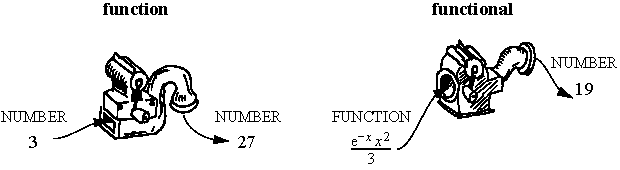
\includegraphics[height=3cm]{fig/fct_fctn.pdf} 
    \caption{函数和泛函的区别,选自 Lancaster, Tom, and Stephen J. Blundell. \emph{Quantum field theory for the gifted amateur}. OUP Oxford, 2014.}
    \label{fig:function_vs_fuctional}
\end{figure}
泛函是什么意思?函数的函数,输入一个函数得到数值,那么函数是数值到数值的映射。DFT 里的泛函是波函数作为输入,我们要找到一个波函数让能量最低。如图 \ref{fig:function_vs_fuctional}。

密度泛函,毫无疑问是指用密度映射能量,即基态能量可以由基态密度唯一确定,这是密度泛函的基本原理。这个原理有什么好处?我们求薛定谔方程,不考虑自旋、时间,波函数 $\psi$ 是 $N$ 个电子 $3N$ 维度的变量,波函数的构造是很复杂的,而且波函数没有物理意义。密度是什么概念?粒子是不可区分的,在任意一点找到电子的概率即密度。如果全空间有 $N$ 个电子,那么密度的全空间积分为 $N$。密度 $\rho$ 是 3 维,但波函数是 $3N$ 维的。密度的求解远比薛定谔方程求解简单。如果能找到密度和能量的映射关系,那么就有更简单的方式求解薛定谔方程。这就是我希望把 DFT 放在变分微扰后面紧接着讲的原因,因为密度泛函理论并没有超出求解薛定谔方程,无非是重构薛定谔方程的方式。变分是寻找尝试波函数,微扰是利用未微扰波函数作为跳板。
DFT 是一种不走寻常路的形式,跳出波函数去寻找密度。

DFT 中最基本的 Hohenberg--Kohn 定理下节课再讲。先尝试从变分推导,
% 2022-11-28 15:03:43  Wenbin Fan @FDU
通过变分看看有没有这种可能性。做\textbf{限制性变分},
\begin{align}
    \langle \psi | \hat H | \psi \rangle |_{\text{min}} = E_0,
\end{align}
% 【】假设知道全空间【?】
这里做了一些理论上的假设,即全体尝试波函数是已知的,那么才能得到上面的等号。

% 2022-11-28 15:04:51  Wenbin Fan @FDU
假如我们有一种很聪明的方式,把波函数的变分空间按所需的方式做任意的组合,我们可以组合出一组 $\{\psi_{\rho_1}\}, \{\psi_{\rho_2}\}, \cdots$ 子空间,它们能给出
密度相同的波函数,
这个子空间构成了 $\big\{\{\psi_{\rho_i}\}\big\} = \{\psi\}$。这种做法仅是从理论上可行,因为波函数空间可以说是无穷大,实际上难以取出所有密度相同的波函数。
% 2022-11-28 15:06:26  Wenbin Fan @FDU
有了这个做法之后,变分就成了最小化具有相同密度下的波函数所对应的能量,
% 找所有的最小。
\begin{align}
\left\{
\begin{array}{l}
\langle \psi_\rho | \hat H |\psi_\rho \rangle|_\text{min} = E[\rho], \\
E[\rho] | _{\text{min}} = E_0
\end{array}
\right.
\end{align}
这里第一行是说,在我们假设变分空间里所有波函数的密度都相同的情况下,最小化``密度函数到能量''这个泛函,最小化得到的是密度函数,第二行是最小化这个密度函数,得到了能量。
换句话说,的确可以将体系能量表示能密度的函数。

% % 2022-11-28 15:07:14  Wenbin Fan @FDU
% 确实可以找出来 $E_0$,

把波函数再展开,
\begin{align}
    E[\rho] = 
\langle    \psi_\rho | \hat T + V_{\mathrm{ee}} + V_{\mathrm{ext}} | \psi_\rho \rangle | _{\text{min}}  
= F[\rho] + V_{\mathrm{ext}}[\rho], 
\end{align}
因为 min 走遍了所有密度相同的波函数,那么动能和库伦项都是相等的,所以动能算符和库伦算符构成了普适泛函。
换句话说,密度泛函的的存在性不需要 HK 定理证明,可以通过限制性变分搜索来证明密度到基态能量的映射关系是存在的。
% 通过限制性搜索,证明密度到能量的映射关系是存在的,
一旦映射关系找到了,我们要去搜索所有的密度,其中最低的能量就是基态能量。如果能构造一个泛函,使得该泛函输出给定密度的最小值能量,那么对密度进行变分可得到体系的基态能量。这个有点超纲了,这里的推导是想说,
如何用变分法从密度给出密度的映射关系,没有任何的数值可行性。

% 2022-11-28 15:10:51  Wenbin Fan @FDU
变分法是构造尝试波函数空间,微扰法是去寻找合适的零级无微扰波函数,密度泛函是为了找到更好的映射关系,进而操作密度而不是波函数得到体系精确的能量。DFT 不对波函数进行操作,但密度不是波函数,密度不包含体系的所有信息,密度不包含微妙的量子耦合等,相当于对体系的全部信息做了取舍,用精度换取计算量,天下没有免费的午餐 no-free-lunch theorem。

上课上到 Dec 19 Mon。还有三次课。我跟大家保证,如果平时作业认真做,最后一定会过的。考试难度只有平时的 70 80\%。本课的出发点不是像高考一样选拔。希望同学们理解化学中背后的物理,当然这离不开数学基础。
